\chapter{Aplikacja wspomagająca ocenę ryzyka kredytowego}

\section{Opis aplikacji}

Zadaniem systemu jest dostarczanie inwestorom informacji niezbędnych do podejmowania decyzji o sprzedaży lub kupnie zadłużenia. Użytkownik będzie miał do dyspozycji następujące moduły:

\begin{itemize}
	\item ogólne statystyki pożyczek z podziałem na poszczególne stany USA,
	\item statystyki pożyczek nie spłacanych w terminie,
	\item model predykcyjny, klasyfikujący pożyczki pod kątem ich zachowania (pozytywne lub negatywne).
\end{itemize}

System został zaimplementowany w formie aplikacji webowej, której poszczególne węzły są uruchamiane w konterach aplikacyjnych Docker, co pozwala na uruchomienie w każdym środowisku, w tym chmurze, niezależnie od konfiguracji serwera oraz innych aplikacji, które są na nim uruchomione. Technologia kontenerów aplikacyjnych została szerzej opisana w następnym rozdziale. 

\section{Wykorzystane technologie}

\subsection{AngularJS}

AngularJS jest frameworkiem napisanym w języku JavaScript utrzymywanym przez firmę Google \cite{angular}. Pozwala na realiację wzorca MVC w aplikacji klienciej obsługiwanej przez przeglądarkę internetową, co ułatwia testowanie, utrzymanie oraz rozwój tej części systemu.  Poza realizacją tego wzroca do najważniejszych cech frameworku należą:

\begin{itemize}
	\item dwukierunkowe wiązanie danych (ang. \textit{two-way binding}) - w przeciwieństwie do standardowych systemów szablonowania nie tylko zmiany w warstwie modelu są na bieżąco renderowane w warstwie widoku, ale również zmiany w warstwie widoku wprowadzone przez użytkownika są automatycznie propagowane do warstwy modelu (Rysunek \ref{angular:two_way}. Pozwala to traktować warstwę widoku jako aktualną projekcję modelu.
		\begin{figure}
			\centering
    		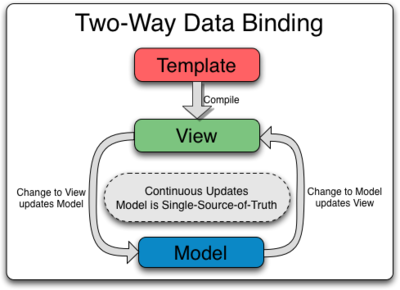
\includegraphics[scale=0.5]{img/Two_Way_Data_Binding.png}
    		\caption{Dwukierunkowe wiązanie danych w AngularJS \cite{angular}.}
    		\label{angular:two_way}
		\end{figure}

	\item odseparowanie logiki aplikacji od maniuplowania strukturą DOM,
	\item odseparowanie warstwy klienckiej od warstwy serwerowej aplikacji webowej,
	\item poprawa testowalności aplikacji klienckiej.
\end{itemize}

\subsection{Node.js}

Node to asynchroniczne, sterowane zdarzeniami środowisko uruchomieniowe języka JavaScript, zaprojektowane z myślą o skalowalnych aplikacjach sieciowych. Prawie żadna z funkcji w Node nie przeprowadza bezpośrednio operacji I/O, co pozwoliło na redykcję ryzyka blokowania procesów \cite{node}.

Node jest zbudowany na podstawie silnika V8 firmy Google, dzięki czemu charakteryzuje się wydajnością prównywalną, a nawet lepszą niż analogiczne aplikacje napisane w języku Java. Zespół pracowników przeprowadził badanie \cite{}